\section{Prototyping and Potential Applications}
\label{sec:proto}

\subsection{Prototype Implementation}
To demonstrate the effectiveness of our design, we implement the proposed \retro\ system. Our prototype is shown in \figref{fig:proto} (a) and (b). The \vitag\ is battery-free and we harvest light energy using solar cell. The size of \vitag\ is $8.2cm\times 5.2cm$, same as a credit card. About two-thirds area is used for solar cells and one-third for the LCD and retro-reflector. 

\begin{figure}[tb!]
\centering
\minipage{.75\columnwidth}
      \subfigure[\vitag Front]{
        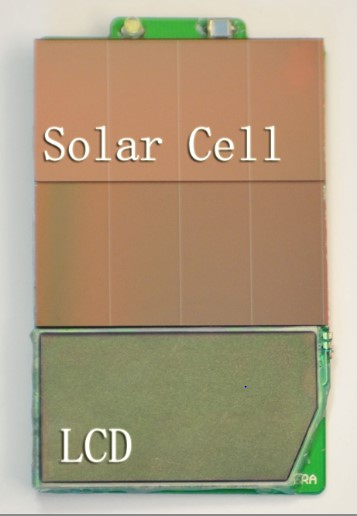
\includegraphics[width=0.45\columnwidth]{tag-front.jpg}
      } 
%      \hskip 1em
      \subfigure[\vitag Back]{
        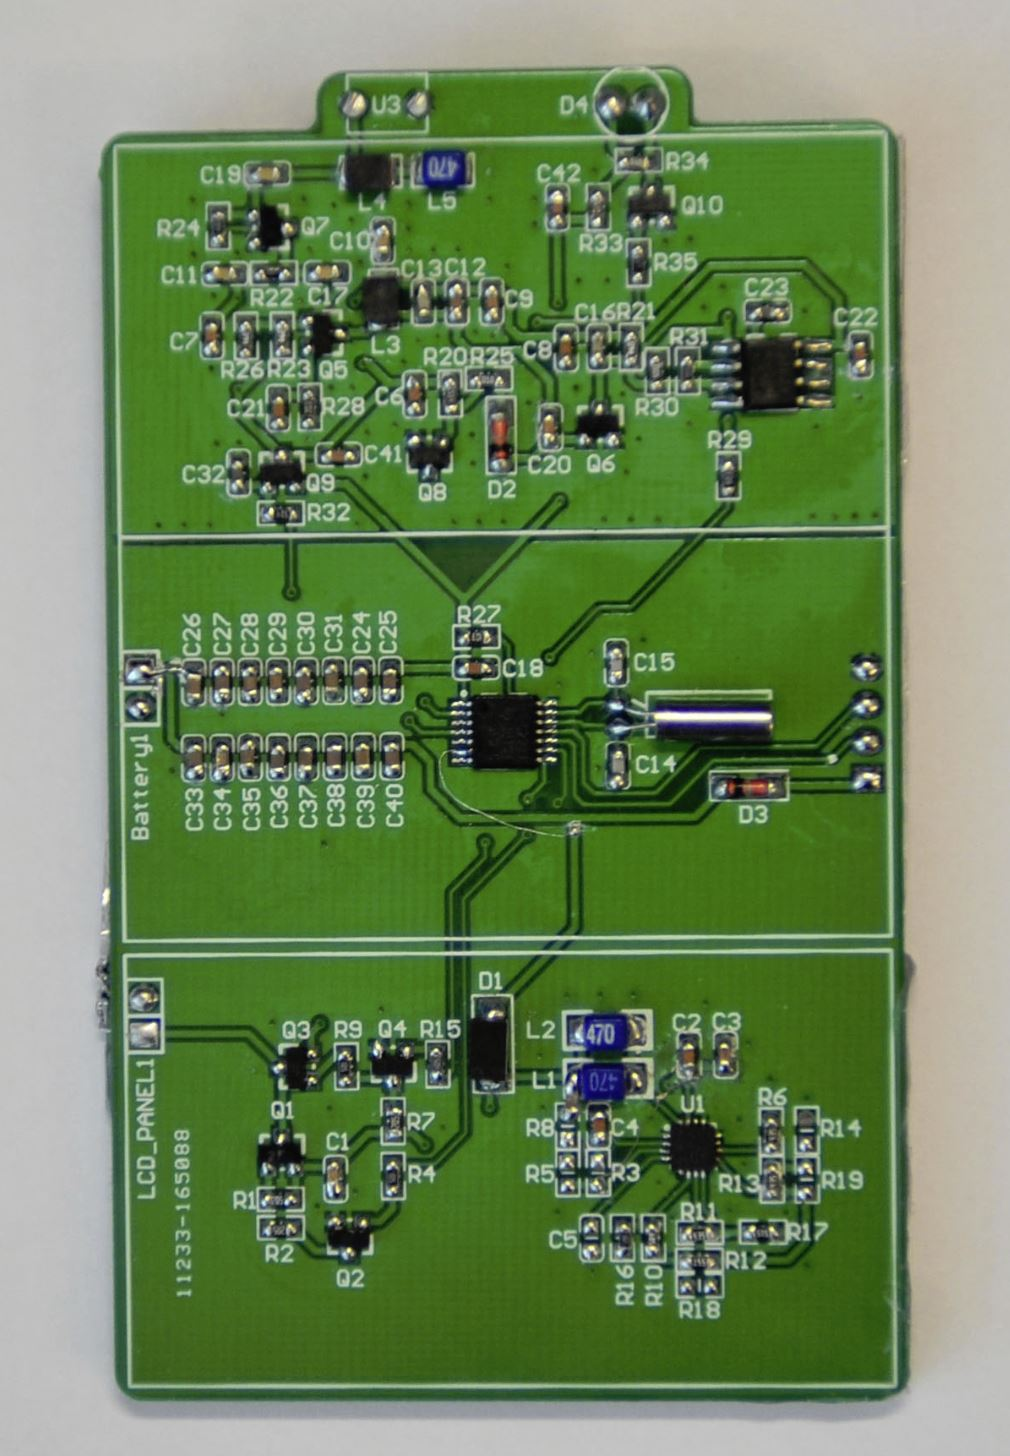
\includegraphics[width=0.45\columnwidth]{tag-back2.jpg}
      } 
%
      \subfigure[Lamp]{
        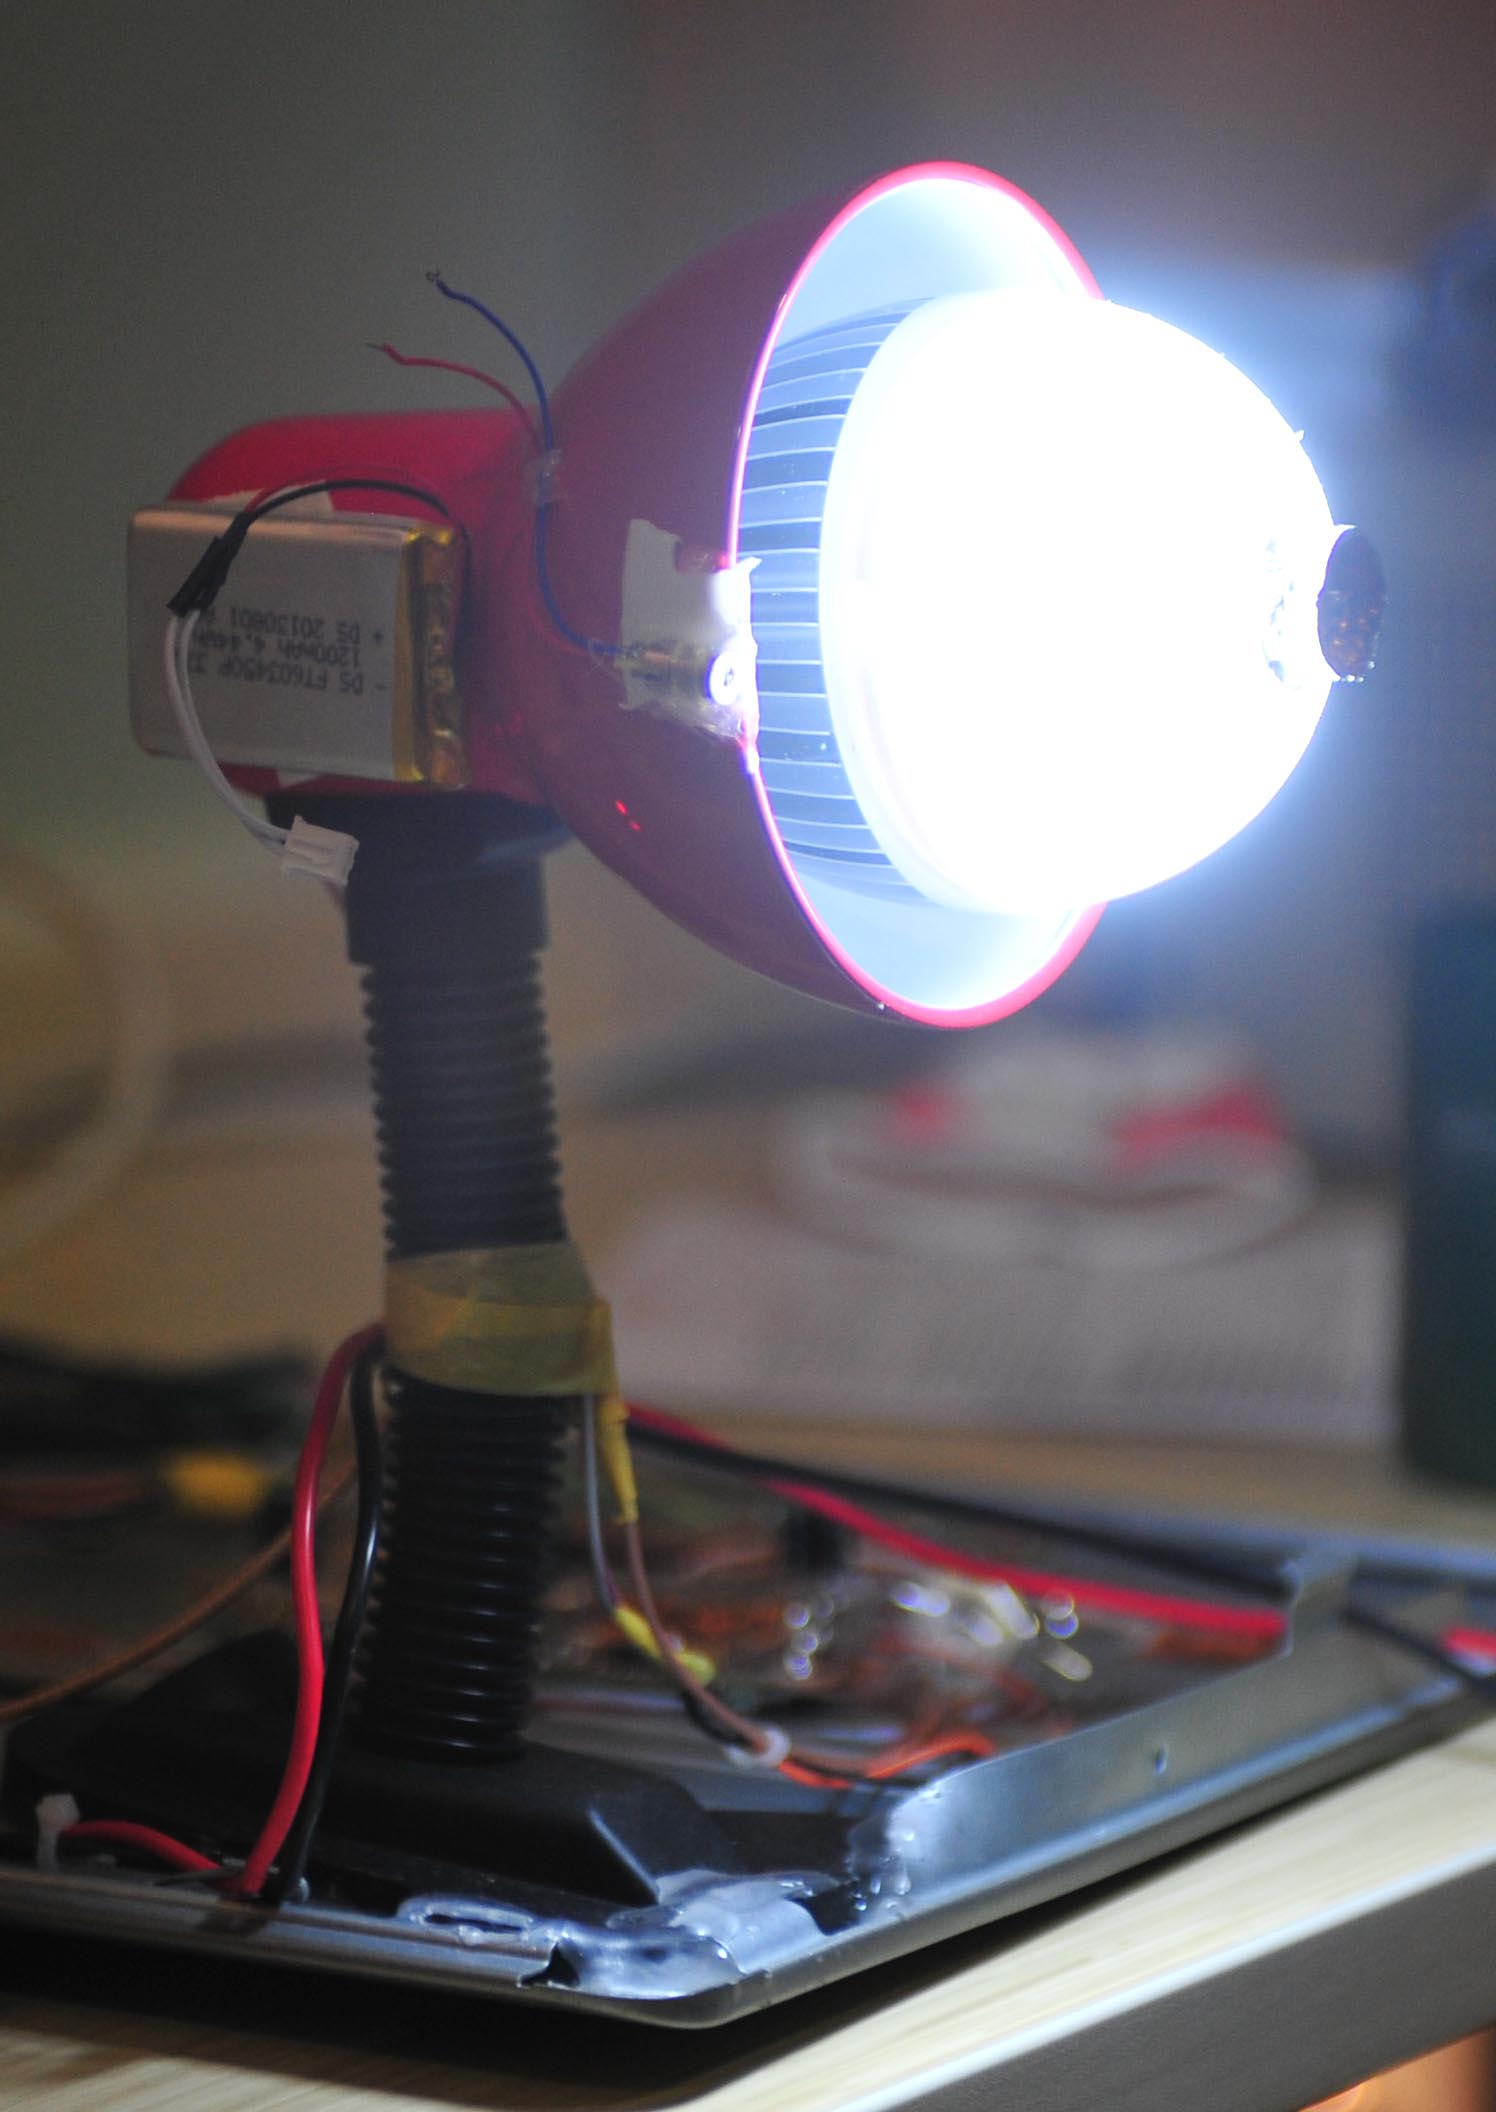
\includegraphics[width=0.47\columnwidth]{reader_lamp_2.jpg}
      } 
%      \hskip 1em
      \subfigure[Flashlight]{
        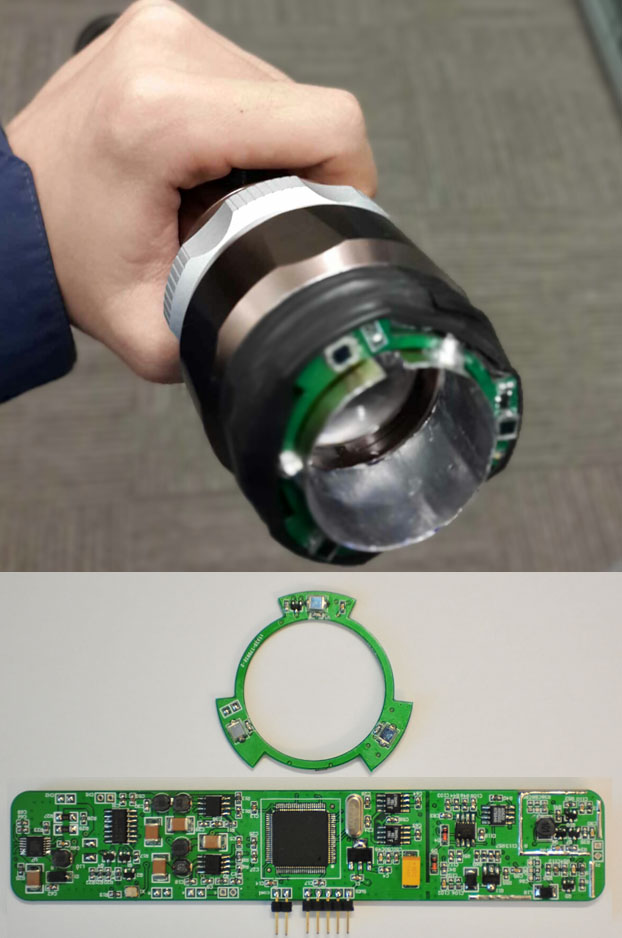
\includegraphics[width=0.44\columnwidth]{reader_torch.jpg}
      } 
\vspace{-1ex}      
\endminipage
\caption{Prototype.}
\label{fig:proto}
%\vspace{-1em}      
\end{figure}

\iffalse
\begin{figure}[!ht]
\centering
\minipage{.7\columnwidth}
      \subfigure[Lamp]{
        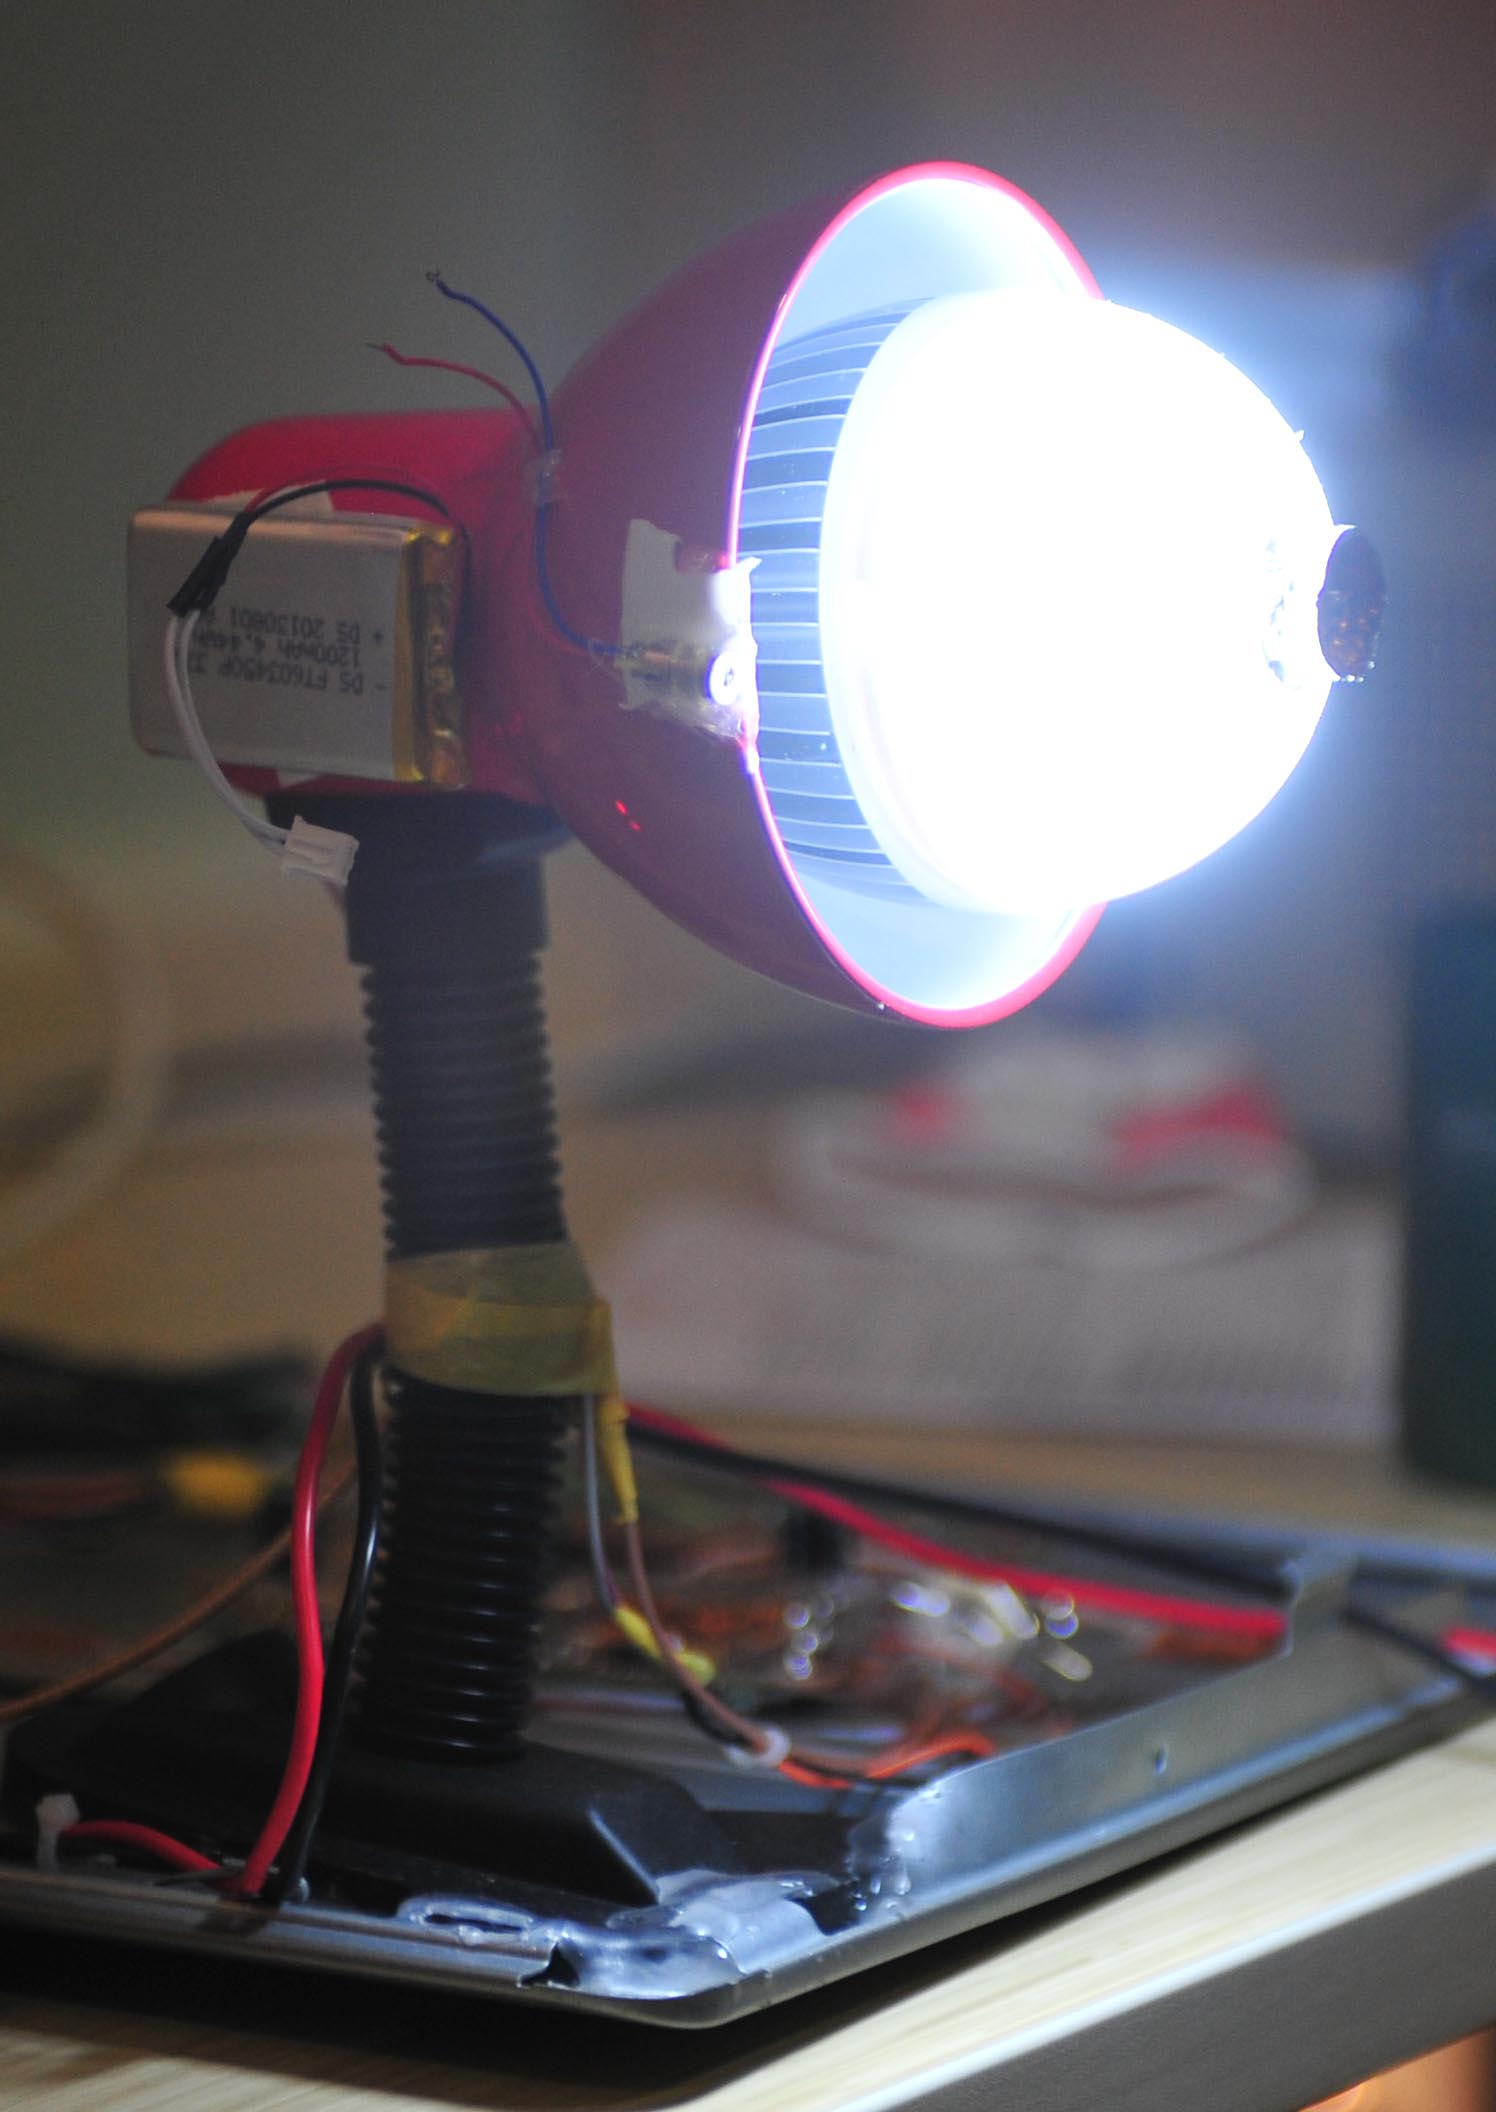
\includegraphics[width=0.47\columnwidth]{reader_lamp_2.jpg}
      } 
%      \hskip 1em
      \subfigure[Flashlight]{
        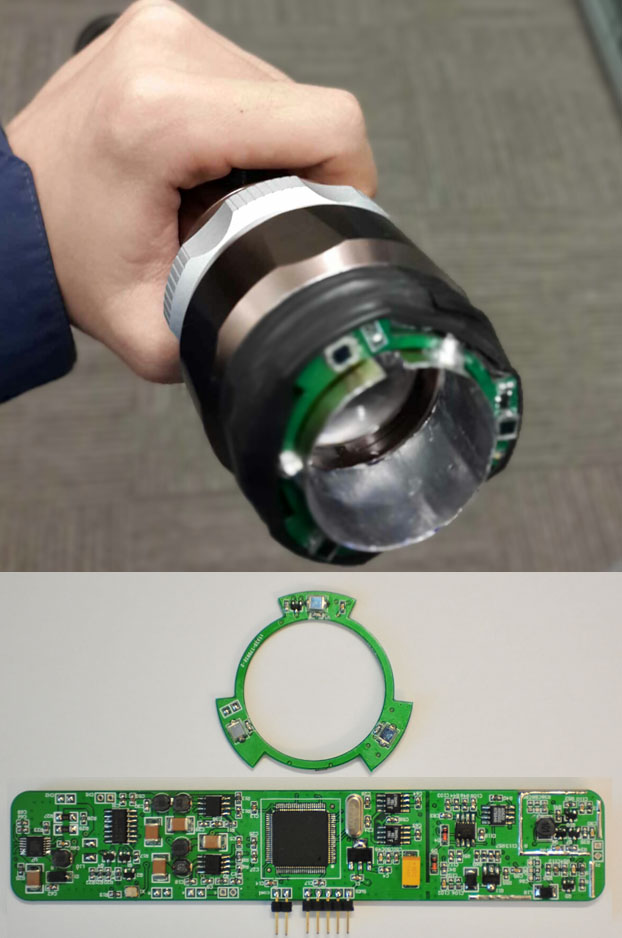
\includegraphics[width=0.44\columnwidth]{reader_torch.jpg}
      } 
\vspace{-1ex}      
\endminipage
\caption{Reader prototype.}
\label{fig:proto_reader}
%\vspace{-1em}      
\end{figure}
\fi

We use the schematics in \figref{fig:sysdiagram} in the implementation with printed circuit boards (PCBs) and off-the-shelf circuit components, which we summarize in Table~\ref{table:components}. The retro-reflector fabric we use is Scotchlite from 3M~\cite{rrsheet}. %We have implemented them as fully reconfigurable platforms, controlled by firmware executed on each individual microcontroller. 

\begin{table}[th]
\begin{center}
\small
\begin{tabular}{| l | l || l | l |}
\hline
\multicolumn{2}{ |c|| }{ \vitag\ } & \multicolumn{2}{ c| }{ \reader\ } \\ \hline\hline

Photodiode 		&  	BPW34 			& 	Photodiode 		&  	SFH213 			\\ \hline
MCU 			&	MSP430G	& 	MCU 			&	LPC4357		\\ \hline	
DC/DC 	&	BQ25504			& 	MOSFET 	&	IRF510			\\ \hline
Comparator		&	TLV2762			& 	Amplifier		&	\footnotesize{LM6172, AD620}			\\ \hline
Transistor		&	S9018 			& 	Transistor		&	\footnotesize{S9018, 2SC3357}			\\ \hline
LCD				&	SF110147 		& 	LED	Bulb			&	Apollo BR30 		\\ \hline
%Reflector 		&	\multicolumn{1}{ |c| } {3M Scotchlite} &  &  \\ \hline
\end{tabular}
\normalfont
%\vspace{-1em}      
\caption{Concrete models of electronic components used in \retro prototype}\label{table:components}
\end{center}
\end{table}

\begin{table}[h]
\begin{center}
\begin{tabular}{| l | l | l |}
\hline
Component\textbackslash Voltage 	& 	2.0V 						& 2.6V 								\\ \hline\hline

\multirow{2}{*}{Receiving Circuit} 	& $43.8\mu A$ 		& $48.4\mu A$ \\
									& ($87.6\mu W$) 	& ($125.8\mu W$) \\ \hline
 
\multirow{2}{*}{Transmitting Circuit} 	& $45.1\mu A$ 		& $36.7\mu A$ \\
									& ($90.2\mu W$) 	& ($95.4\mu W$) \\ \hline
									
\multirow{2}{*}{Total} 	& $91.9\mu A$ 		& $90.0\mu A$ \\
									& ($183.8\mu W$) 	& ($234.0\mu W$) \\ \hline									
\end{tabular}
%\vspace{-1em}
\caption{Overall and component-wise energy consumption of \vitag.}\label{table:energy}
\end{center}
\end{table}

The \reader\ is implemented in two forms. The first one is a lamp reader, which is modified from an $12W$ white LED lamp, as shown in \figref{fig:proto}(c). We put the light sensor inside the center of front surface of the lamp and isolate it with copper foil to reduce the leakage from the LED light. The second one is a flashlight reader, shown in \figref{fig:proto}(d). It uses a $3W$ LED as the transmitter. Three light sensors are used to improve the SNR. %The lamp reader is designed to work with large FOV but relatively short distance(about 2.5m, 50\degree), while the falshlight reader is designed to work with long distance with a narrower FOV (about 10.6m, 8.5\degree).


The energy consumption of \vitag is related to the voltage output of solar cell. We measure the overall and component-specific energy consumption for \vitag for two typical operating voltages, as shown in Table~\ref{table:energy}. The measurement shows that the \vitag prototype indeed achieves ultra-low power consumption. With such low power consumption, we are able to drive it by harvesting light energy using only small solar cells.

%\todo{If calculation supports that a single cell battery can last for years, then we can add some argument here saying that: In our prototype, two-thirds area is occupied by the solar cell. If smaller tags is desired, we can use cell battery. Our calculation indicate that a single xxx cell battery can last xxx long under xxx traffic.}

%MCU generated signal modulates the light and then we use a power MOSFET to implement an RF power amplifier. The amplified signal is sent to the bulb to be transmitted.

%The implementation of the \vitag\ receiver starts with a PIN photodiode as the light sensor. The captured signal is sent to a series of triode amplifiers and bandpass filters, after which the signal enters the high-gain demodulator.
%This demodulated signal is then sent to a comparator implemented using a TLV2762 operational amplifier, before the decoding process with an MSP430.

%In the \vitag\ transmitting phase, an SF110147 LCD is used, covering a retro-reflector fabric. For the energy reuse module, we use a diode to prevent the waste of the current and directs it to the recycling capacitor, and we use a BQ25504 to implement the DC-DC converter.

%The \reader\ receiver uses an SFH213 light sensor, parallel with an LC resonant circuit. It's followed by an impedance matching circuit and then the tuned differential amplifier, whose gain is controlled by the Cortex M4, aiming to decouple the RF interferences. Then we implement another two RF amplifiers using high frequency transistors. Sequentially, the active envelope detector is implemented using an LM6172 operational amplifier, along with 1N60 diodes. Finally, the signal passes through a baseband amplifier, arriving at the MCU ADC port.



%We notice that for a given lighting environment and a target \vitag size, there ought to be an optimal division between the area for solar cell and that for retro-reflector. 

%\p{liqul: we should have a dedicated section like "Trade-off of sizes" discussing how we partition the constrained board size into two retro-reflector and solar cell. The intuition is that we should not assign too much space to either side. There should be an optimal partitioning. Not sure if our current design is optimal.}

\iffalse
%\subsubsection{Solar Cell Size v.s. Communication Range}
\vskip 0.05in\noindent{\it Experiments.} We test how far the tag can be reached as we cover part of the solar cell.

\vskip 0.05in\noindent{\it Results.} Fig.~\ref{fig:solar} shows the solar cell area does not affect the communication range within a certain region. \hl{there is a threshold, above which succeed, below which fail}


\begin{figure}[tb!]
\centering
\includegraphics[width=0.7\columnwidth]{../evaluation/SolarCellSize_Range.eps}
\vskip -0.05in
\caption{\footnotesize{\bf Solar Cell Size V.S. Communication Range.} \todo{Need to explain the units of X-axis.}.}
\label{fig:solar}
\vskip -0.05in
\end{figure}

%\subsubsection{Reflector Size v.s. Communication Range}

\vskip 0.05in\noindent{\it Experiments.} We test how far the tag can be reached as we cover part of the retro-reflector.

\vskip 0.05in\noindent{\it Results.} Fig.~\ref{fig:retro} shows \hl{area covered proportional to range}

\begin{figure}[tb!]
\centering
\includegraphics[width=0.7\columnwidth]{../evaluation/ReflectorSize_Range.eps}
\vskip -0.05in
\caption{\footnotesize{\bf Retro-Reflector Size V.S. Communication Range.} \todo{Need to explain the units of X-axis. It's area, should be square cm.}.}
\label{fig:retro}
\vskip -0.05in
\end{figure}
\fi

\subsection{Potential Applications}
The low power duplex \retro system has many potential application scenarios. 

\paragraph{Home sensor bearer} Sensors such as motion, temperature, humidity and other sensors can be integrated with \vitag. Sensor readings can be streamed to a \reader-capable lighting LED. Such an application would benefit from the battery-free property of \vitag: deployment is extremely simple and sensors can remain untethered afterwards.   

\paragraph{Visible-light identification (VLID)} Taking visible light as the communicating media, VLID has many advantages over radio-frequency based identification systems, such as can achieve distant communication with battery free Tags, immune to electromagnetic interference, and more secure, thus it has the potential of replacing RFID in many scenarios such as in warehouses, storage and transportation systems.

\paragraph{Interactive road side traffic signs} The battery-free design of \vitag can be applied to road-side signs. Cars can communicate with them using LED headlights. Similarly, it can be used for automatic tollgate. 

\paragraph{NFC communication/payment} The use of visible light and the directional reflection property of the retro-reflector makes it a securer and faster means than other wireless NFC system.  The tag size can made smaller if only for short range communication. 
